\documentclass[11pt, letter]{amsart}


\usepackage[margin=1in]{geometry}
\usepackage{amsthm}
\usepackage{amsmath}
\usepackage{amssymb}
\usepackage{enumerate}
\usepackage[inline]{enumitem}

\newtheorem*{theorem*}{Theorem}
\newtheorem*{lemma*}{Lemma}
\theoremstyle{definition}
\newtheorem{problem}{Problem}[]
\newtheorem{exercise}{Exercise}[]
\newtheorem*{definition*}{Definition}

\usepackage{tikz}
\usetikzlibrary{calc}
\definecolor{OwlRed}{RGB}{ 255, 92, 168}
\definecolor{OwlGreen}{RGB}{ 90, 168, 0}
\definecolor{OwlBlue}{RGB}{ 0, 152, 233}
\definecolor{OwlYellow}{RGB}{ 242, 147, 24}
\colorlet{OwlViolet}{OwlRed!50!OwlBlue}
\colorlet{OwlBrown}{OwlRed!50!OwlGreen}
\colorlet{OwlOrange}{OwlRed!50!OwlYellow}
\colorlet{OwlCyan}{OwlGreen!50!OwlBlue}
\colorlet{pink}{OwlRed}
\colorlet{green}{OwlGreen}
\colorlet{blue}{OwlBlue}
\colorlet{yellow}{OwlYellow}
\colorlet{violet}{OwlViolet}
\colorlet{brown}{OwlBrown}
\colorlet{orange}{OwlOrange}
\colorlet{cyan}{OwlCyan}
\newcommand{\cB}{\ensuremath{\mathcal B}}


\title[Math 4032: Homework \#6\qquad Due April 21 at 1:59pm]{Math 4032: Homework \#6\\
  Due April 21 at 1:59pm}


\begin{document}


\maketitle

This assignment is on combinatorial design theory.  Relevant background material for this assignment is covered in Chapters 5 and 12 of the Jukna book and Chapters 9 and 13 of the Matou\v{s}ek--Ne\v{s}et\v{r}il book.  However, note that some material covered in class is not in either text.

\begin{itemize}
\item You are strongly encouraged to typeset your homework solutions using \LaTeX.
\item Acknowledge collaborations as noted in the syllabus.
\item The following problems are optional exercises not to be turned in.  Problems to be turned in for a grade begin on the next page.  
\end{itemize}

\begin{exercise}
  Find a set of three MOLS of order $4$.
\end{exercise}

\begin{exercise}~
  \begin{enumerate}[label=(\alph*)]
  \item Construct a symmetric Latin square of order $5$ with $1, 2, 3, 4, 5$ appearing in that order on the diagonal.
  \item Construct Steiner triple system of orders $13$ and $15$. \textit{Hint: For the order $15$, use the Latin square from part (a).  For the order $13$, use the Latin square which is the addition table of $\mathbb Z_2\times \mathbb Z_2$.}
  \end{enumerate}
\end{exercise}


\begin{exercise}
  Use three MOLS of order $4$ to construct an affine plane of order $4$.
\end{exercise}

\begin{exercise}
  Use the operation described in Problem 4 to construct an order-$3$ projective plane from the order-$3$ affine plane depicted in Problem 3.
\end{exercise}

\begin{exercise}
  Show that there is no $5$-$(16, 7, 1)$ design.
\end{exercise}

\clearpage

Recall that a \textit{transversal} in a Latin square $L = (\ell_{i,j})_{i,j\in[n]}$ of order $n$ is a set of $n$ entries $(i_1, j_1), \dots, (i_n, j_n) \in [n]\times [n]$ such that each row, column, and symbol appears exactly once, i.e.\ $i_1, \dots i_n$ are distinct, $j_1, \dots, j_n$ are distinct, and $\ell_{i_1,j_1}, \dots, \ell_{i_n, j_n}$ are distinct.  A \textit{perfect matching} in a hypergraph $(V, \cB)$ (sometimes called a \textit{parallel class} in the context of design theory) is a set $M \subseteq \cB$ of pairwise disjoint edges such that that every vertex is in exactly one edge in $M$, i.e.\ $V = \bigcup_{A \in M}A$.  The hypergraph is \textit{resolvable} if there is a decomposition of $\cB$ into pairwise disjoint perfect matchings / parallel classes.
\begin{problem}Let $L = (\ell_{i,j})_{i,j\in[n]}$ be an order-$n$ Latin square.  Prove that the following are equivalent:
  \begin{enumerate}[label=(\alph*)]
  \item $L$ has an orthogonal mate;
  \item $L$ has a decomposition into $n$ pairwise disjoint transversals;
  \item the graph $G = ([n]\times [n], E)$, where
    \begin{equation*}
      E = \left\{\left\{(i,j),(i',j')\right\}\in \binom{[n]\times[n]}{2} : i = i',~j = j',~\text{or}~\ell_{i,j} = \ell_{i',j'}\right\},
    \end{equation*}
    has chromatic number $n$.
  \item the hypergraph $(V, \cB)$ where $V = \{(\{\textsc{ROW}\}\times [n]) \cup (\{\textsc{COL}\}\times [n]) \cup (\{\textsc{SYM}\}\times [n])\}$ and
    \begin{equation*}
      E = \left\{\left\{(\textsc{ROW}, i), (\textsc{COL}, j), (\textsc{SYM}, k)\right\} : \ell_{i,j} = k\right\}
    \end{equation*}
    is resolvable.
  \end{enumerate}
\end{problem}

% \begin{proof}
% Let assumptions be as in the problem statement.\\
% (a) $\Longleftrightarrow$ (b): Let us assume that the latin square $L$ has an orthogonal mate $L'$. That is to say that any pair $(a_{ij}, b_{ij})$ for $a_{ij}\in L, b_{ij}\in L'$ is distinct. Then we can follow any distinct symbol in one latin square, let's use $L'$, to then find a transversal in the other, $L$. And since there are $n$ symbols to follow in $L'$, we can then partition $L$ into $n$ distinct transversals that are disjoint as desired. Alternatively, consider if $L$ has a decomposition into $n$ pairwise disjoint transversals. We can use each of these transversals and label each with a single symbol to create an orthogonal latin square to $L$. Essentially following the above process in the other order to create and orthogonal mate. Therefore, $L$ has an orthogonal mate as desired.
% \\
% (a) $\Longleftrightarrow$ (c): If we use the fact that given that a latin square $L$ has an orthogonal mate implied that $L$ can be divided into $n$ pairwise disjoint transversals as above, if we color each of the $n$ disjoint traversals one color, then we will find that once all of these traversals are colored $n$ different colors that it will construct the graph $G$ as desired, and have chromatic number $n$ as desired. Alternatively, if we begin with the graph $G$ as defined where $G$ has chromatic number $G$, then we can just label all the vertices of $G$ with the same symbol which would be the orthogonal mate to a latin square $L$ and we can use the process from above to construct the orthogonal mate as desired.
% \\
% (a) $\Longleftrightarrow$ (d): If we assume that $L$ is a latin square with orthogonal mate, then we know that $L$ can be decomposed into $n$ pairwise disjoint transversals. We can follow the algorithm similar to the colorings above, if we group the disjoint transversals into edges, we can construct the hypergraph as specified in the problem statement as desired. Alternatively if we assume that we have a hypergraph as defined in the problem statement, then we can take each of these pairwise disjoint perfect matchings and labels them a single symbol which would be the orthogonal mate of the latin square $L$ and we can just simply derrange it to create $L$ as desired.
% \end{proof}

\clearpage
An \textit{isomorphism} from a hypergraph $(V_1, \cB_1)$ to a hypergraph $(V_2, \cB_2)$ is a bijection $f : V_1 \rightarrow V_2$ such that $B_1 \in \cB_1$ if and only if $\{f(v) : v\in B_1\} \in \cB_2$.
\begin{problem}~
  \begin{enumerate}[label=(\alph*)]
  \item Prove that every Steiner triple system of order $7$ is isomorphic to the Fano plane (below, left). \textit{Hint: Prove that any two triples of an order-$7$ Steiner triple system intersect.}

    % \begin{proof}
    %     We will first create a na\"ive construction of a steiner triple system of order 7. We will label the sets of points $\{x_1, ..., x_7\}$, then we can define the blocks $\{x_1, x_2, x_3\}, \{x_1, x_4, x_5\},\\ \{x_1, x_6, x_7\}, \{x_2, x_6, x_5\}, \{x_3, x_6, x_4\}, \{x_3, x_7, x_5\}, \{x_2, x_4, x_7\}$. It is simple to see that this construction meets the needs of the steiner triple system of order 7, and it is simple to also see that this would map to the Fano plane, and that any two of these triples intersect. If there exists another steiner triple system of order 7 that is not isomorphic to this construction, that would mean that it would have at least one triple disjoint from another triple, i.e. it doesn't share an element with the other triple. Let us define such triples, WLOG, as $B_1 = \{x_1, x_2, x_3\}$ and the triple it is disjoint from as $B_2 = \{x_4, x_5, x_6\}$. Thus, this leave one other point not included in either of these triples $x_7$. However, if we attempt to construct a triple that would include any pair with $x_7$, it would require one of the elements be from $B_1$ and the other form $B_2.$ If we follow a construction in this manner, we will be able to create 3 more triples. This means that we are able to contain $15$ pairs which is $6$ pairs shy of the the total $\binom{7}{2} = 21$ pairs. Therefore, since there is no way for us to construct an order-$7$ steiner triple system by defining that there is a pair of disjoint triples, then we know that any two triples of an order-$7$ steiner triple system intersect. Thus this implies that every steiner triple system of order 7 is isomorphic to the Fano plane as desired.
    % \end{proof}
  
  \item Prove that every Steiner triple system of order $9$ is isomorphic to the order-$3$ affine plane (below, right). \textit{Hint: Prove that for every triple in an order-$9$ Steiner system, there are only two triples disjoint from it, and moreover, these two are also disjoint.}

    % \begin{proof}
    %     We will first create a construction of a steiner triple system of order 9. We will label the set of points $\{x_1, ..., x_9\}$ to represent the 9 points, and we will define the block to be $\{x_1, x_2, x_3\}, \{x_4, x_5, x_6\}, \{x_7, x_8, x_9\}, \{x_1, x_4, x_7\}, \{x_2, x_5, x_8\}, \{x_3, x_6, x_9\}, \{x_1, x_5, x_9\},\\ \{x_2, x_6, x_7\}, \{x_3, x_4, x_8\}, \{x_2, x_4, x_9\}, \{x_3, x_5, x_7\}, \{x_1, x_6, x_8\}$ which is the representation that makes up the affine plane of order 3. We can inspect this and see that there are in fact 4 sets of 3 disjoint triples (proved in problem 3) an example of which is $\{x_1, x_2, x_3\}, \{x_4, x_5, x_6\},\\ \{x_7, x_8, x_9\}$. Now assume for the sake of contradiction that there in fact does exist another steiner triple system of order 9 that is not isomorphic to the affine plane of order 3 (the formulation above). This is to say that such a formulation would have a set of either more than $3$ disjoint triples or a set of fewer such triples. Well it is simple to see that the situation in which there are more disjoint triples is not possible becuase in order to have 4 disjoint triples, it would require 12 points which would no longer be in a steiner triple system of order 9. So that implies that we would need to have 2 or fewer disjoint triples. Let us first deal with the case in which there are no disjoint triples. We will state that one of the block be $\{x_1, x_2, x_3\}$ WLOG, and in order for all of the other triples to not be disjoint from this one, they must all contain a point from this triple. However, when we attempt to construct the rest of the steiner triple system in this manner, we will be unable to obtain all other pairs of points without creating another disjoint triple. This is because while we will be able to construct triples that will contain all pairs with $x_1$ it will not allow us to create pairs between other elements. For example, if we took $\{x_1, x_2, x_3\}, \{x_1, x_4, x_7\}, \{x_1, x_5, x_8\}, \{x_1, x_6, x_9\}, \{x_2, x_4, x_9\}, \{x_2, x_5, x_7\}, \{x_2, x_6, x_8\},\\ \{x_3, x_6, x_7\}, \{x_3, x_4, x_8\}, \{x_3, x_5, x_9\}$ we will create all pairs that include $x_1, x_2, x_3$, but we won't be able to create the pairs of $\{x_4, x_5\}$ just as an example of a problem. Therefore, we know we must have at least two disjoint triples. Let us define such triples as $\{x_1, x_2, x_3\}$ and $\{x_4, x_5, x_6\}$ WLOG. Then we need to construct all triples such that they will then intersect these two triples, thus meaning that it must contain a point from the first block and a point from the second block. However, when we try to create a triple that contains a pair with any of the three elements not in either of the first two predetermined triple, we will be unable to create a block that is not disjoint from both blocks implying that we must have a set of three disjoint triples such is isomorphic to the affine plane of order 3 as desired.
    % \end{proof}
  
  \end{enumerate}
\end{problem}
\begin{center}
  \begin{minipage}{.5\linewidth}
    \centering
    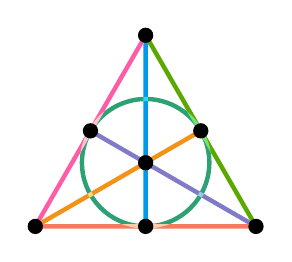
\begin{tikzpicture}
      \tikzstyle{vtx}=[draw, thick, fill, circle, scale=.5];
      \tikzstyle{hyperedge}=[ultra thick];

      \pgfdeclarelayer{foreground} 
      \pgfdeclarelayer{background}
      \pgfsetlayers{background,%
        foreground%
      }
      \pgfmathsetmacro{\rad}{1.618}
      \begin{pgfonlayer}{foreground}
        \node[vtx] (hub) at (0, 0) {};
        \node[vtx] (top) at (90:\rad) {};
        \node[vtx] (left) at (210:\rad) {};
        \node[vtx] (right) at (-30:\rad) {};
        \node[vtx] (tl) at ($(top)!.5!(left)$) {};
        \node[vtx] (tr) at ($(top)!.5!(right)$) {};
        \node[vtx] (b) at ($(left)!.5!(right)$) {};
      \end{pgfonlayer}

      \begin{pgfonlayer}{background}
        \begin{scope}[transparency group]
          \begin{scope}[blend mode=screen]
            \draw[pink, hyperedge] (left) -- (tl) -- (top);
            % \draw (left.150) -- (tl.150) -- (top.150);
            % \draw (left.-30) -- (tl.-30) -- (top.-30);

            \draw[green, hyperedge] (right) -- (tr) -- (top);
            % \draw (right.30) -- (tr.30) -- (top.30);
            % \draw (right.-150) -- (tr.-150) -- (top.-150);

            \draw[blue, hyperedge] (b) -- (hub) -- (top);
            % \draw (b.180) -- (hub.180) -- (top.180);
            % \draw (b.0) -- (hub.0) -- (top.0);
            
            \draw[yellow, hyperedge] (left) -- (hub) -- (tr);
            % \draw (left.120) -- (hub.120) -- (tr.120);
            % \draw (left.-60) -- (hub.-60) -- (tr.-60);
            
            \draw[violet, hyperedge] (right) -- (hub) -- (tl);
            % \draw (right.60) -- (hub.60) -- (tl.60);
            % \draw (right.-120) -- (hub.-120) -- (tl.-120);

            \draw[orange, hyperedge] (left)  -- (b) -- (right);
            % \draw (left.-90)  -- (b.-90) -- (right.-90);
            % \draw (left.90)  -- (b.90) -- (right.90);
            
            % \draw (tl) -- (b) -- (tr);
            \draw[cyan, hyperedge] (0, 0) circle (.5*\rad);
          \end{scope}
        \end{scope}
        
      \end{pgfonlayer}
    \end{tikzpicture}%\\Projective plane%

  \end{minipage}%
  \begin{minipage}{.5\linewidth}
    \centering
    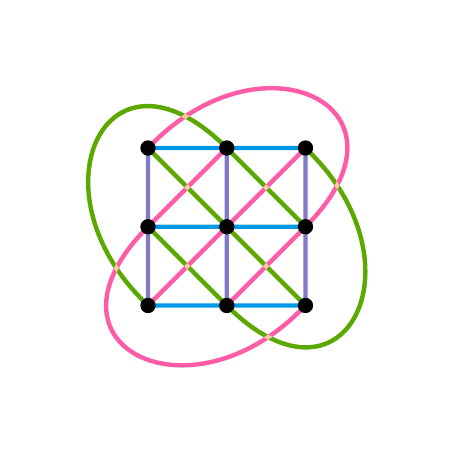
\begin{tikzpicture}
      \tikzstyle{vtx}=[draw, thick, fill, circle, scale=.5];
      \tikzstyle{hyperedge}=[ultra thick];

      \tikzstyle{hidden}=[opacity=0];
      \tikzstyle{col1} = [opacity=.8, fill=blue];
      \tikzstyle{col2} = [opacity=.8, fill=pink];
      \tikzstyle{col3} = [opacity=.8, fill=green];
      \tikzstyle{col4} = [opacity=.8, fill=orange];

      \pgfdeclarelayer{foreground} 
      \pgfdeclarelayer{background}
      \pgfsetlayers{background,%
        main,%
        foreground%
      }

      \begin{pgfonlayer}{foreground}
        \node[vtx] (c) at (0, 0) {};
        \node[vtx] (r) at (1, 0) {};
        \node[vtx] (l) at (-1, 0) {};
        \node[vtx] (top) at (0, 1) {};
        \node[vtx] (tr) at (1, 1) {};
        \node[vtx] (tl) at (-1, 1) {};
        \node[vtx] (bottom) at (0, -1) {};
        \node[vtx] (br) at (1, -1) {};
        \node[vtx] (bl) at (-1, -1) {};
      \end{pgfonlayer}
      
      \begin{pgfonlayer}{background}
        \begin{scope}[transparency group]
          \begin{scope}[blend mode=screen]
            \pgfmathsetmacro{\len}{1.5}
            \draw[hyperedge, blue] (bl) -- (bottom) -- (br);
            \draw[hyperedge, blue] (l) -- (c) -- (r);
            \draw[hyperedge, blue] (tl) -- (top) -- (tr);
            
            \draw[hyperedge, pink] (bl) -- (c) -- (tr);
            \draw[hyperedge, pink] (bottom) -- (r.center) .. controls ($(r) + (\len, \len)$) and ($(tl) + (\len, \len)$) .. (tl);
            \draw[hyperedge, pink] (top) -- (l.center) .. controls ($(l) + (-\len, -\len)$) and ($(br) + (-\len, -\len)$) .. (br);
            
            \draw[hyperedge, green] (tl) -- (c) -- (br);
            \draw[hyperedge, green] (l) -- (bottom.center) .. controls ($(bottom) + (\len, -\len)$) and ($(tr) + (\len, -\len)$) .. (tr);
            \draw[hyperedge, green] (r) -- (top.center) .. controls ($(top) + (-\len, \len)$) and ($(bl) + (-\len, \len)$) .. (bl);
            
            \draw[hyperedge, violet] (bl) -- (tl);
            \draw[hyperedge, violet] (br) -- (tr);
            \draw[hyperedge, violet] (bottom) -- (top);
          \end{scope}
        \end{scope}

      \end{pgfonlayer}
    \end{tikzpicture}
  \end{minipage}
\end{center}
\clearpage

Recall the definition of \textit{parallel class} and \textit{resolvable} from Problem 1.  An \textit{affine plane of order $q$} is a hypergraph $(V, \cB)$ where
\begin{itemize}
\item $|V| = q^2$,
\item $\cB \subseteq \binom{V}{q}$ (the elements of $\cB$ are called \textit{lines}), and
\item every two distinct $u,v\in V$ are in a unique line $B \in \cB$.
\end{itemize}
(An order-$3$ affine plane is depicted to the right in Problem 2.)
\begin{problem}
  Prove that every affine plane is resolvable.  More generally, prove that
  \begin{itemize}
  \item there are $q + 1$ parallel classes containing $q$ lines each and
  \item any two lines from different parallel classes intersect.
  \end{itemize}
  \textit{Hint: Prove that every vertex is in $q + 1$ lines and that there are $q^2 + q$ lines.  Each vertex is contained in one line from every parallel class, so the set of $q + 1$ lines containing some fixed vertex contains a representative for each parallel class.}
\end{problem}

% \begin{proof}
%     Let assumptions be as in the problem statement. Let us pick a particular vertex $v\in V$. We know that there are then $q^2 - 1$ other points and since $v$ must make a pair with each of these other points, we know then that this blocks will then have $q - 1$ other vertices on them. Thus, we know that there are then $\frac{q^2 - 1}{q-1} = q + 1$ blocks containing the point $v$. By the definition of a parallel class, we know that any particular point $p$ is in only one block in that parallel class. Thus, we have $q + 1$ different blocks that we can choose from to define the parallel classes, and since we can define the parallel class using any of these lines, we then know that we have $q + 1$ parallel classes as desired. Furthermore, each of these parallel classes will have $n$ blocks.
% \end{proof}

\clearpage

A \textit{projective plane} of order $q$ is a hypergraph $(V, \cB)$ where
\begin{itemize}
\item $|V| = q^2 + q + 1$,
\item $\cB \subseteq \binom{V}{q + 1}$ (the elements of $\cB$ are called \textit{lines}), and
\item every two distinct $u,v\in V$ are in a unique line $B \in \cB$.
\end{itemize}
(An order-$2$ projective plane is depicted to the left in Problem 2.)
\begin{problem} This problem shows that a projective plane of order $q$ exists if and only if an affine plane of order $q$ exists.
  \begin{enumerate}
  \item Let $(V, \cB)$ be a projective plane of order $q$, let $L \in B$, let $V' = V \setminus L$, and let $\cB' = \{L' \setminus L : L' \in \cB, L' \neq L\}$.  Prove that $(V', \cB')$ is an affine plane of order $q$.  \textit{Note: The removed line is called the ``line at infinity''.}

% \begin{proof}
%     Let assumptions be as in the problem statement. In order for this $(V', \cB')$ to indeed be an affine plane, we need to show that it satisfies all the conditions of an affine plane. It is simple to see that $|V'| = |V| - |L|$ and by definition of a projective plane we know that $|V'| = |V| - |L| = q^2 + q + 1 - (q + 1) = q^2$ which is the correct number of vertices for an affine plane of order $q$. Similarly if we remove $L$ from the set of blocks and it's respective points from the remaining blocks, and since each line that intersects $L$ can only do so one time by definition since if it contained more than one then one pair would be in more than one line which is not allowed. Thus, we find that the size $|L'| = |L| - 1 = q + 1 - q = q$ as desired by the definition of an affine plane. Lastly, since the condition that every pair is in a unique line, which will be maintained when we remove points. Additionally for the property stated in the previous of having $q + 1$ parallel classes, we see if we have two lines in the original graph, if they are incident on each other at some point $p \in L$, when we remove $L$ these two will become parallel in the resulting affine plane, and this will apply to all other lines that are incident on each other at points on $L$. 
% \end{proof}
  
  \item Let $(V, \cB)$ be an affine plane of order $q$, and let $Y$ be the set of its parallel classes (which has size $q + 1$ by the previous problem).  For each $L \in \cB$, let $L^* = L \cup \{C\}$, where $C$ is the parallel class containing $L$.  Let $V' = V \cup Y$, and let
    \begin{equation*}
      \cB' = \{Y\} \cup \{L^* : L \in \mathcal B\}.
    \end{equation*}
    Prove that $(V', \cB')$ is a projective plane of order $q$.  \textit{Note: This operation is called `adding a line at infinity'.}

% \begin{proof}
%     Let assumptions be as in the problem statement. We want to check if $(V', \cB')$ is a resulting projective plane of order $q$. By the definition of $V'$ we know that we are going to add $q + 1$ vertices to the graph, each vertex representing each of the $q + 1$ parallel classes of the original affine plane. Thus we find that $|V'| = |V| + |Y| = q^2 + q + 1$ which is what is desired for a projective plane of order $q$. Similarly, we will extend each line to the new $q + 1$ points if that line is in the parallel class represented by each of the points. This means, each of the lines in a parallel class, which are currently parallel in the affine plane sense, will now be incident on each other at the point that represents their appropriate parallel class. This then implies that each line will now gain an extra vertex making $|L^*| = |L| + 1 = q + 1$ which is the appropriate size for a projective plane. Lastly, we know that we won't have two line that share the same pair because for the original $q$ vertices, they already did not share any pairs, and when we add the new $q + 1$ vertices, any lines that will now become incident on each other will only be incident at that point since they were parallel in the original affine plane as per the definition of the respective parallel classes. Therefore, since this result meets all the properties of a projective plane, we know that $(V', \cB')$ is a projective plane of order $q$ as desired.
% \end{proof}
    
  \end{enumerate}
\end{problem}
\clearpage

\begin{problem}
  Let $(V, \cB)$ be a $2$-$(n, k, \lambda)$ design, and let $\cB' = \{V \setminus B : B \in \cB\}$.  Prove that $(V, \cB')$ is a $2$-$(n, n - k, \lambda')$ design for some $\lambda'$.  What is $\lambda'$ (in terms of $n$, $k$, and $\lambda$)?
\end{problem}

% \begin{proof}
%     Let assumptions be as in the problem statement, then we know that each of the original $B\in \cB$ has $k$ vertices. Thus by definition we also know that the new blocks in $\cB'$ will be of size $n - k$ if we define them to be the vertices that were not in the original block $B$, so we do know that $(V, \cB')$ is $n-k$ uniform. Hence implying that this is now a $2-(n, n-k, \lambda')$ design for some $\lambda'$ as desired. Now we are curious to find out the value of $\lambda'$, i.e. how many blocks each pair of vertices show up in. This value $\lambda'$ is simple to see as a case of inclusion-exclusion where we need the number of blocks $|\cB|$ and we need to remove the number of blocks that contain any one point $x\in V$ and another point that makes a pair with it $y\in V$ $r$ and we need to add back the number of blocks that contain both points $\lambda$. Thus we find that $\lambda' = \lambda - 2r + b$ for $r$ is the number of blocks a single point appears in and $b$ is the number of blocks there are.
% \end{proof}


\end{document}

%%% Local Variables:
%%% mode: latex
%%% TeX-master: t
%%% End:
